\documentclass[12pt]{article}
\usepackage[usenames]{color} %used for font color
\usepackage{amsmath,amssymb,amsthm,amsfonts} %maths
\usepackage[utf8]{inputenc} %useful to type directly accentuated characters
\usepackage{hyperref}
\usepackage[margin=0.3in]{geometry}
\usepackage{graphicx}

\usepackage{booktabs}
\usepackage{pgfplots}
\usepackage{pgfplotstable}
\usepackage{siunitx}
\usepackage{multirow}
\usepackage{makecell}


\newtheorem*{claim}{Claim}  % environment for claim

% environment for code
\usepackage{xcolor}
\definecolor{dimgray}{gray}{0.9}

\usepackage{listings}
\lstdefinestyle{R-code}{
	language=R,
	basicstyle=\small\ttfamily,
	commentstyle=\ttfamily\color{brown},
	numbers=left,
	numberstyle=\ttfamily\color{gray}\footnotesize,
	stepnumber=1,
	numbersep=5pt,
	backgroundcolor=\color{dimgray},
	showspaces=false,
	showstringspaces=false,
	showtabs=false,
	frame=single,
	tabsize=2,
	captionpos=b,
	breaklines=true,
	breakatwhitespace=false,
	title=\lstname,
	escapeinside={},
	keywordstyle={\color{blue}},
	morekeywords={}
}
\lstdefinestyle{R-output}{
	basicstyle = \scriptsize\sffamily,
	backgroundcolor=\color{white},
	showspaces=false,
	showstringspaces=false,
	showtabs=false,
	frame=single,
	tabsize=4,
	captionpos=b,
	breaklines=true,
	breakatwhitespace=false,
}



% TikZ for flowchart
\usepackage{tikz, pgfplots}
\usetikzlibrary{shapes.geometric, arrows}

\tikzstyle{process} = [rectangle, rounded corners, minimum width=1cm, minimum height=1cm, text centered, draw=black, fill=orange!30]
\tikzstyle{arr} = [thick,->,>=stealth]



\newcommand\independent{\protect\mathpalette{\protect\independenT}{\perp}}
\def\independenT#1#2{\mathrel{\rlap{$#1#2$}\mkern2mu{#1#2}}}

\newtheoremstyle{problemstyle}  							% <name>
        {3pt}                                               % <space above>
        {3pt}                                               % <space below>
        {\normalfont}                               		% <body font>
        {}                                                  % <indent amount}
        {\bfseries}                 						% <theorem head font>
        {\normalfont\bfseries.}         					% <punctuation after theorem head>
        {.5em}                                          	% <space after theorem head>
        {}                                                  % <theorem head spec (can be left empty, meaning `normal')>
\theoremstyle{problemstyle}

\newtheorem{problem}{}
\newtheorem{solution}{Solution}
\newtheorem*{solution*}{Solution}

\newcommand{\createcontingencytable}[4]{ %
% #1=table name
% #2=first column name
% #3=new row sum name
% #4=new column sum name
\pgfplotstablecreatecol[
    create col/assign/.code={% In each row ... 
        \def\rowsum{0}
        \pgfmathtruncatemacro\maxcolindex{\pgfplotstablecols-1}
        % ... loop over all columns, summing up the elements
        \pgfplotsforeachungrouped \col in {1,...,\maxcolindex}{
            \pgfmathsetmacro\rowsum{\rowsum+\thisrowno{\col}}
        }
        \pgfkeyslet{/pgfplots/table/create col/next content}\rowsum
    }
]{#3}{#1}%
%
% Transpose the table, so we can repeat the summation step for the columns
\pgfplotstabletranspose[colnames from={#2},input colnames to={#2}]{\intermediatetable}{#1}
%
% Sums for each column
\pgfplotstablecreatecol[
    create col/assign/.code={%
        \def\colsum{0}
        \pgfmathtruncatemacro\maxcolindex{\pgfplotstablecols-1}
        \pgfplotsforeachungrouped \col in {1,...,\maxcolindex}{
            \pgfmathsetmacro\colsum{\colsum+\thisrowno{\col}}
        }
        \pgfkeyslet{/pgfplots/table/create col/next content}\colsum
    }
]{#4}\intermediatetable
%
% Transpose back to the original form
\pgfplotstabletranspose[colnames from=#2, input colnames to=#2]{\contingencytable}{\intermediatetable}
}
%

\makeatletter
\newcommand*\bigcdot{\mathpalette\bigcdot@{.5}}
\newcommand*\bigcdot@[2]{\mathbin{\vcenter{\hbox{\scalebox{#2}{$\m@th#1\bullet$}}}}}
\makeatother

\def\ed { \stackrel{d}{=} }
\def\convd { \stackrel{d}{\rightarrow} }
\def\corr{\mathrm{corr}}
\def\normal{\mathcal{N}}
\def\R{\mathbb{R}}
\def\Pr{\mathbb{P}}
\def\M{\mathcal{M}}
\def\F{\mathcal{F}}

\newcommand{\indep}{\mathrel{\text{\scalebox{1.07}{$\perp\mkern-10mu\perp$}}}}


\begin{document}

\begin{center}{\large\textbf{Homework 5} \hfill \large \textit{Categorical Data Analysis, S. S. Mukherjee, Fall 2019}} 
\end{center}
\hrule\hrule\vskip3pt
Topics:  Correspondence analysis, causal inference, structural equation models\hfill Due on December 12, 2019\vskip3pt
\hrule\hrule\vskip3pt\noindent
Name of student: Subhrajyoty Roy\\
Roll number: MB1911
\vskip3pt\noindent	
%%%%%%%%%%%%%%%%%%%%%%%%%%%%%%%%%%%%%%%%%%%%%%%%%%
% Problem 1
%%%%%%%%%%%%%%%%%%%%%%%%%%%%%%%%%%%%%%%%%%%%%%%%%%
\begin{problem}
\textbf{Correspondence analysis} \hfill [10]\vskip3pt\noindent
% Problem statement
\begin{enumerate}
    \item[(a)] Let $r_k$, $s_k$ be the row, column indices corresponding to the $k$-th largest singular value $\sqrt{\lambda_k}$ of $C$. Show that
    \begin{align*}
    \mathbb{E}_I r_{kI} &= 0,\quad \mathbb{E}_J s_{kJ} = 0, \text{ and}\\
    \mathrm{Var}_I(r_{kI}) &= \mathrm{Var}_J(s_{kJ}) = \frac{\lambda_k}{x_{\bigcdot\bigcdot}},  
    \end{align*}
    where $I$ and $J$ are random row and column indices from the corresponding marginal distributions.

    \item[(b)]Express the conditional distributions $(\frac{x_{ij}}{x_{i\bigcdot}})_{j = 1}^p$ and $(\frac{x_{ij}}{x_{\bigcdot j}})_{i = 1}^n$ in terms of the indices $r$ and $s$.
    \item[(c)] Apply correspondence analysis (including visualization) on the contingency table given \href{https://soumendu041.gitlab.io/teaching/courses/cda2019/problems/writers_data.csv}{here}, and interpret the result. (Each row of the table corresponds to a text sample by a writer, whereas columns correspond to the occurrence of particular letters. Thus the $(i, j)$-th cell gives the frequency of the $j$-th letter in the $i$-th text sample.)
\end{enumerate}  
\end{problem}
%%%%%%%%%%%%%%%%%%%%%%%%%%%%%%%%%%%%%%%%%%%%%%%%%%
% Solution to problem 1
%%%%%%%%%%%%%%%%%%%%%%%%%%%%%%%%%%%%%%%%%%%%%%%%%%
\begin{solution*}
% Write your solution here:

\begin{enumerate}
	\item[(a)] Let us denote; $a = \left( x_{1\bigcdot}, x_{2\bigcdot}, \dots x_{n\bigcdot} \right)^{\top}$ and $A$ be the diagonal matrix with the entries $x_{i\bigcdot}$. 
	We know that, $r_k = \sqrt{\lambda_k} A^{-1/2}\gamma_k$, where $\gamma_k$ is the eigenvector of $CC^{\top}$ corresponding to $k$-th largest eigenvalue. Then,
	\begin{align*}
		\mathbb{E}_I r_{kI} & = \sum_{i=1}^{n} \frac{x_{i\bigcdot}}{x_{\bigcdot\bigcdot}}r_{ki}\\
		& = \frac{1}{x_{\bigcdot\bigcdot}} a^{\top}r_k\\
		& = \frac{1}{x_{\bigcdot\bigcdot}} a^{\top}\sqrt{\lambda_k} A^{-1/2}\gamma_k\\
		& = \frac{1}{\sqrt{\lambda_k}x_{\bigcdot\bigcdot}} \sqrt{a}^{\top}\lambda_k\gamma_k\\
		& = \frac{1}{\sqrt{\lambda_k}x_{\bigcdot\bigcdot}} \sqrt{a}^{\top}CC^{\top}\gamma_k\\
		& = 0 \text{, since} \sqrt{a}^{\top}C = 0
	\end{align*}
	
	Similarly, as $C\sqrt{b} = 0$, where $b = \left( x_{\bigcdot 1}, x_{\bigcdot 2}, \dots x_{\bigcdot p} \right)^{\top}$, we have $\mathbb{E}_J s_{kJ} = 0$.
	
	For the variance, note that;
	\begin{align*}
		\mathrm{Var}_I(r_{kI}) & = \sum_{i=1}^{n} \frac{x_{i\bigcdot}}{x_{\bigcdot\bigcdot}}r_{ki}^2 \text{, since the expectation is 0 by previous argument}\\
		& = \frac{1}{x_{\bigcdot\bigcdot}} r_k^{\top} A r_k\\
		& = \frac{1}{x_{\bigcdot\bigcdot}} \lambda_k \gamma_k^{\top} A^{-1/2}AA^{-1/2} \gamma_k\\
		& = \frac{\lambda_k}{x_{\bigcdot\bigcdot}} \gamma_k^{\top}\gamma_k\\
		& = \frac{\lambda_k}{x_{\bigcdot\bigcdot}}
	\end{align*}
	where the last equality follows from the fact that due to Singular Value Decomposition, $\gamma_k$'s form an orthonormal basis and hence $\Vert \gamma_k \Vert = 1$.
	
	In a similar way, we also have, $\mathrm{Var}_J(s_{kJ}) = \frac{\lambda_k}{x_{\bigcdot\bigcdot}}$.
	
	
	\item[(b)] We know that;
	\begin{align*}
		r_{ki} & = \frac{\sqrt{x_{\bigcdot\bigcdot}}}{\sqrt{\lambda_k}} \sum_{j}\frac{x_{ij}}{x_{i\bigcdot}}s_{kj}\\
		s_{kj} & = \frac{\sqrt{x_{\bigcdot\bigcdot}}}{\sqrt{\lambda_k}} \sum_{i}\frac{x_{ij}}{x_{\bigcdot j}}r_{ki}	
	\end{align*}
	
	Letting $a_{ij} = \frac{x_{ij}}{x_{i\bigcdot}}$ and $b_{ij} = \frac{x_{ij}}{x_{\bigcdot j}}$, and dividing the equation by each other, we obtain;
	
	$$\frac{r_{ki}}{s_{kj}} = \dfrac{\sum_{j} a_{ij} s_{kj} }{\sum_{i} b_{ij} r_{ki} }$$
	
	which implies;
	
	\begin{equation}
		\label{eqn:cond-1}
		\sum_{j} a_{ij} s_{kj}^2  = \sum_{i} b_{ij} r_{ki}^2
	\end{equation}
	
	Also note that; 
	\begin{equation}
		\label{eqn:cond-2}
		\sum_{j} a_{ij} = \sum_{i} b_{ij} = 1
	\end{equation}
	
	Note that both the equation \ref{eqn:cond-1} and \ref{eqn:cond-2} are true for any $i = 1, 2, \dots n$ used on the left hand side and for any $j = 1, 2, \dots p$ used on the right hand side. Therefore, we consider the following vector of size $2np$,
	
	$$\textbf{P} = \begin{bmatrix}
	a_{11}\\
	a_{12}\\
	\dots\\
	a_{1p}\\
	a_{21}\\
	\dots \\
	a_{np}\\
	b_{11}\\
	\dots \\
	b_{np}\\
	\end{bmatrix}$$
	
	which consists of the entries made from the conditional probabilities.
	
	Let us denote the Kronecker product between two matrices $A$ and $B$ by $A\otimes B$, denote the matrix of all $1$'s of size $n\times n$ by $J_n$, and the identity matrix of order $n$ by $I_n$. Also, let $\textbf{S}_k$ is the diagonal matrix consists of the entries $s_{kj}^2$ and $\textbf{R}_k$ is the diagonal matrix consists of the entries $r_{ki}^2$.
	
	Now, note that, equation \ref{eqn:cond-1} and \ref{eqn:cond-2} reduces to the following matrix equation;
	
	$$\begin{bmatrix}
	I_n \otimes J_p & -(J_n \otimes I_p)\\
	I_n \otimes \textbf{S}_1 & -(\textbf{R}_1 \otimes I_p)\\
	\dots & \dots\\
	I_n \otimes \textbf{S}_m & -(\textbf{R}_m \otimes I_p)
	\end{bmatrix}_{mnp \times 2np} \textbf{P}_{2np \times 1} = \textbf{0}_{mnp \times 1}$$
	
	where $m$ is the number of indexes present in the correspondence analysis. Denoting the $mnp\times 2np$ order matrix as $\mathbb{M}$, we note that, the vector $P$ can be chosen from the null space of the matrix $\mathbb{M}$. Also, note that, this only ensures that, $\sum_{j} a_{i^\ast j} = \sum_{i} b_{ij^\ast}$ holds for every $i^\ast$ and $j^\ast$, however, the condition that the sum is actually equal to one can be obtained through dividing the entries by appropriate constant.
	
	
	\item[(c)] We first read the data into \texttt{R}.
	
	\begin{lstlisting}[style = R-code]
		data <- read.csv('./writers_data.csv')
		ctab <- as.matrix(data[, -1])
		rownames(ctab) <- data[, 1]
		ctab
	\end{lstlisting}
	\begin{lstlisting}[style = R-output]
		                B  C  D  F  G  H  I  L  M  N  P  R  S  U  W  Y
		CharlesDarwin1 34 37 44 27 19 39 74 44 27 61 12 65 69 22 14 21
		CharlesDarwin2 18 33 47 24 14 38 66 41 36 72 15 62 63 31 12 18
		CharlesDarwin3 32 43 36 12 21 51 75 33 23 60 24 68 85 18 13 14
		ReneDescartes1 13 31 55 29 15 62 74 43 28 73  8 59 54 32 19 20
		ReneDescartes2  8 28 34 24 17 68 75 34 25 70 16 56 72 31 14 11
		ReneDescartes3  9 34 43 25 18 68 84 25 32 76 14 69 64 27 11 18
		ThomasHobbes1  15 20 28 18 19 65 82 34 29 89 11 47 74 18 22 17
		ThomasHobbes2  18 14 40 25 21 60 70 15 37 80 15 65 68 21 25  9
		ThomasHobbes3  19 18 41 26 19 58 64 18 38 78 15 65 72 20 20 11
		MaryShelley1   13 29 49 31 16 61 73 36 29 69 13 63 58 18 20 25
		MaryShelley2   17 34 43 29 14 62 64 26 26 71 26 78 64 21 18 12
		MaryShelley3   13 22 43 16 11 70 68 46 35 57 30 71 57 19 22 20
		MarkTwain1     16 18 56 13 27 67 61 43 20 63 14 43 67 34 41 23
		MarkTwain2     15 21 66 21 19 50 62 50 24 68 14 40 58 31 36 26
		MarkTwain3     19 17 70 12 28 53 72 39 22 71 11 40 67 25 41 17
	\end{lstlisting}
	
	We use \texttt{FactoMineR} package to perform the correspondence analysis of the above data and make necessary visualization plots.
	
	\begin{lstlisting} [style = R-code]
		library(FactoMineR)
		fit <- CA(ctab, ncp = 14, graph = TRUE)
		head(fit$eig)
	\end{lstlisting}
	
	\begin{lstlisting}[style = R-output]
		       eigenvalue percentage of variance cumulative percentage of variance
		dim 1 0.018582834              37.265385                          37.26539
		dim 2 0.009425336              18.901250                          56.16663
		dim 3 0.007100377              14.238855                          70.40549
		dim 4 0.005292075              10.612547                          81.01804
		dim 5 0.003628482               7.276435                          88.29447
		dim 6 0.002153008               4.317569                          92.61204
	\end{lstlisting}
	
	It seems the first 6 components alone accounts for more than $90\%$ of the variation measured by Pearsonian chi-square.
	
	\begin{lstlisting}[style = R-code]
		plot(1:14, fit$eig[,3], type = "b", lwd = 2, xlab = "Number of Eigenvalues to keep", 
		ylab = "Percentage of Chi-square explained")
		abline(h = 80, col = "blue", lty = 2)
		abline(h = 90, col = "purple", lty = 2)
		abline(h = 95, col = "red", lty = 2)
	\end{lstlisting} 
	
	\begin{center}
		\includegraphics[width=\linewidth]{screeplot.jpeg}
	\end{center}

	The screeplot shows a better view of the proportion of variation explained based on number of eigenvalues used. We see that using only 4 dimensions, we can capture about $80\%$ of the variability, while using 7 dimension, we get to capture more than $95\%$ of the variability measured through Pearson's chi-square.
	
	\begin{center}
		\includegraphics[width=\linewidth]{caplot.jpeg}
	\end{center}
	
	The above biplot shows the representation using only first 2 dimensions. We find that the letter \textbf{B} and \textbf{C} appears more often in \textbf{Charles Darwin}'s writings, while the letter \textbf{D} appears more often in \textbf{Mark Twain}'s writings. Another interesting thing is that the writings of same author's tend to cluster together due to similar patterns. 
	
	
\end{enumerate}

\end{solution*}
\vskip3pt
%%%%%%%%%%%%%%%%%%%%%%%%%%%%%%%%%%%%%%%%%%%%%%%%%%
% Problem 2
%%%%%%%%%%%%%%%%%%%%%%%%%%%%%%%%%%%%%%%%%%%%%%%%%%
\begin{problem}
\textbf{Causal inference} \hfill [5]
\vskip3pt\noindent
% Problem statement
Suppose that $C_i, i = 0, 1,$ have continuous and strictly increasing CDFs $F_i, i = 0, 1,$ and that the treatment is randomly assigned. Assume that the consistency relationship $Y = C_X$ holds. Using data $(Y_i, X_i)_{i = 1}^n$, show that it is possible to consistently estimate the following measure of causal effect
\[
    \theta_m = \mathrm{median}(C_1) - \mathrm{median}(C_0).
\]
\end{problem}
%%%%%%%%%%%%%%%%%%%%%%%%%%%%%%%%%%%%%%%%%%%%%%%%%%
% Solution to problem 2
%%%%%%%%%%%%%%%%%%%%%%%%%%%%%%%%%%%%%%%%%%%%%%%%%%
\begin{solution*}
% Write your solution here.

Before proceeding with the problem, we first consider the following claim.

\begin{claim}
	Let $X_1, X_2, \dots X_n$ be i.i.d. samples from a continuous distribution function $F$ with median $\xi$ defined as $\Pr_F(X \geq \xi) = \Pr_F(X \leq \xi) = 0.5$. Then the sample median $\hat{\xi}_n$ is consistent for population median $\xi$, i.e. $\hat{\xi}_n\xrightarrow{P} \xi$ as $n\rightarrow \infty$.
\end{claim}
\begin{proof}
	To prove consistency, choose $\epsilon > 0$. It is enough to show that;
	$\Pr_F(\hat{\xi}_n - \xi > \epsilon ) \rightarrow 0$ as $n \rightarrow \infty$, since then by symmetry it will follow that $\Pr_F(\hat{\xi}_n - \xi < -\epsilon ) \rightarrow 0$ as $n \rightarrow \infty$, i.e. $\Pr_F(\vert \hat{\xi}_n - \xi \vert > \epsilon ) \rightarrow 0$ as $n \rightarrow \infty$, which proves the consistency.
	
	Now,
	\begin{align*}
		\Pr_F(\hat{\xi}_n - \xi > \epsilon ) & = \Pr_F(\hat{\xi}_n > \xi + \epsilon)\\
		& = \Pr_F\left(Z_n \geq (n+1)/2 \right)
	\end{align*}
	where $Z_n$ denotes the number of samples which exceeds the value $(\xi + \epsilon)$. Note that, $Z_n \sim \text{Binomial}(n, p)$, where $p = \Pr_F(X > \xi + \epsilon) < 0.5$, as $\xi$ is the median. Hence,
	\begin{align*}
		\Pr_F(\hat{\xi}_n - \xi > \epsilon ) & = \Pr_F\left(Z_n \geq (n+1)/2 \right)\\
		& = \Pr_F\left(Z_n - np \geq (n+1)/2 - np\right)\\
		& = \Pr_F\left(Z_n - np \geq n(0.5 - p) + 1/2\right)\\
		& \leq \Pr_F\left(Z_n - np \geq n(0.5 - p) \right)\\
		& \leq \frac{\text{Var}(Z_n)}{n^2(0.5 - p)^2} \quad \text{from Chebyshev's inequality}\\
		& = \frac{p(1-p)}{n(0.5 - p)^2}\\
		& \rightarrow 0 \quad \text{, as} n \rightarrow \infty 
	\end{align*}
	This proves the claim.
\end{proof}

Now, moving on, let $\hat{\xi}_1$ denotes the sample median of $Y$ in the subpopulation where $X = 1$, and let  $\hat{\xi}_0$ denotes the sample median of $Y$ in the subpopulation where $X = 0$. Clearly, $\hat{\xi}_1 \xrightarrow{P} \xi_1$, where $\xi_1$ is the population median of the conditional distribution of $Y$ given $X = 1$, i.e. the conditional distribution of $C_1$ given $X = 1$. But note that, due to random assignment $X \indep C_i$, and hence the conditional distribution of $C_1$ given $X = 1$ is same as the unconditional distribution of $C_1$. Therefore, $\hat{\xi}_1 \xrightarrow{P} \mathrm{median}(C_1)$. 

In a similar way, $\hat{\xi}_0 \xrightarrow{P} \mathrm{median}(C_0)$. Now, applying Slutsky's theorem, we conclude that $(\hat{\xi}_1 - \hat{\xi}_0) \xrightarrow{P} \theta_m$. Since, both $\hat{\xi}_1$ and $\hat{\xi}_0$ are quantities based on the data, hence it is possible to consistently estimate $\theta_m$, the causal effect.



\end{solution*}
%%%%%%%%%%%%%%%%%%%%%%%%%%%%%%%%%%%%%%%%%%%%%%%%%%
% Problem 3
%%%%%%%%%%%%%%%%%%%%%%%%%%%%%%%%%%%%%%%%%%%%%%%%%%
\begin{problem}
    \textbf{Structural equation models} \hfill [5]
    \vskip3pt\noindent
    % Problem statement
    Consider the structural equations
    \begin{align*}
        Y &= aX + bW + \epsilon_1, \\
        X &= c Z + dW + \epsilon_2.
    \end{align*}
    Here $X, Y, Z, W$ are observed/manifest variables, and $\epsilon_i, i = 1, 2,$ are error variables which represent unexplained random disturbances. Draw the corresponding path diagram and identify the endogenous and exogenous variables. Express the covariance matrix $\Sigma$ of the observed variables in terms of the other parameters $\theta$ in the model, i.e. the path coefficients and the error variances. (Assume that $\mathrm{cov}(\epsilon_1, \epsilon_2) = \mathrm{cov}(\epsilon_1, X) = \mathrm{cov}(\epsilon_1, W) = \mathrm{cov}(\epsilon_2, Z) = \mathrm{cov}(\epsilon_2, W) = 0$.) Describe how you may estimate $\theta$ from the sample covariance matrix $S$.  
\end{problem}
%%%%%%%%%%%%%%%%%%%%%%%%%%%%%%%%%%%%%%%%%%%%%%%%%%
% Solution to problem 2
%%%%%%%%%%%%%%%%%%%%%%%%%%%%%%%%%%%%%%%%%%%%%%%%%%
\begin{solution*}
% Write your solution here.

The path diagram of the given structural equation model is as follows;\\

\begin{center}
	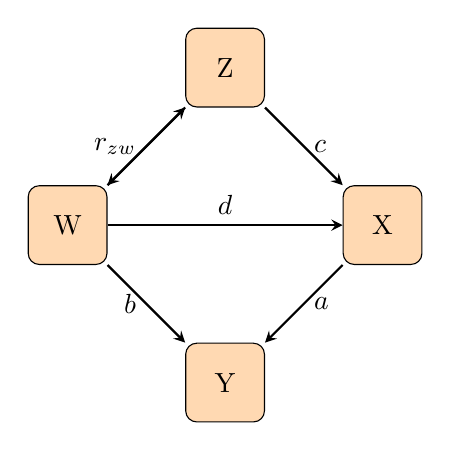
\begin{tikzpicture}[node distance=2cm]
	
	\node (z) [process] {Z};
	\node (w) [process, below of=z, xshift = -2cm] {W};
	\node (x) [process, right of=w, xshift = 2cm] {X};
	\node (y) [process, below of=w, xshift = 2cm] {Y};
	
	\draw [arr] (z) -- node[anchor = east] {$r_{zw}$} (w);
	\draw [arr] (w) -- (z);
	\draw [arr] (z) -- node[anchor = west] {$c$} (x);
	\draw [arr] (w) -- node[anchor = south] {$d$} (x);
	\draw [arr] (w) -- node[anchor = east] {$b$} (y);
	\draw [arr] (x) -- node[anchor = west] {$a$} (y);
	
	\end{tikzpicture}	
\end{center}

The corresponding endogenous variables are $X$ and $Y$, and the corresponding exogenous variables are $Z$ and $W$.

Let us denote the covariance between any variable $A$ and $B$ by $\sigma_{AB}$, and hence the generic symbol for variance of $A$ would be given by $\sigma_{AA}$. To get the covariance matrix we consider the following expression for its elements;

\begin{align*}
	\sigma_{XX} & = c^2 \sigma_{ZZ} + d^2 \sigma_{WW} + 2cd \sigma_{ZW} + \sigma_{\epsilon_1}\\
	\sigma_{XZ} & = c \sigma_{ZZ} + d \sigma_{ZW}\\
	\sigma_{XW} & = c \sigma_{ZW} + d \sigma_{WW}\\
	\sigma_{YY} & = a^2 \sigma_{XX} + b^2 \sigma_{WW} + 2ab \sigma_{XW} + \sigma_{\epsilon_2}\\
	& = (a^2c^2)\sigma_{ZZ} + (a^2d^2 + b^2 + 2abd) \sigma_{WW} + (2a^2cd + 2abc) \sigma_{ZW} + \sigma_{\epsilon_2}\\
	& = (a^2c^2)\sigma_{ZZ} + (ad + b)^2 \sigma_{WW} + 2ac(ad + b) \sigma_{ZW} + \sigma_{\epsilon_2}\\
	\sigma_{YZ} & = a \sigma_{XZ} + b \sigma_{ZW}\\
	& = ac \sigma_{ZZ} + (ad + b) \sigma_{ZW}\\
	\sigma_{YW} & = a \sigma_{XW} + b \sigma_{WW}\\
	& = ac \sigma_{ZW} + (ad + b) \sigma_{WW}\\
	\sigma_{YX} & = a \sigma_{XX} + b \sigma_{XW}\\
	& = ac^2 \sigma_{ZZ} + (ad^2+bd) \sigma_{WW} + (2acd + bc) \sigma_{ZW} + a\sigma_{\epsilon_1}
\end{align*}

We have corresponding sample covariance estimate for $\sigma_{AA}$ denoted by $s_{AA}$. Then, we first consider the equations;

\begin{align}
	\label{eqn:c-and-d}
	s_{XZ} & = c s_{ZZ} + d s_{ZW}\\
	s_{XW} & = c s_{ZW} + d s_{WW}
\end{align}

The linear equations \ref{eqn:c-and-d} can be solved to estimate values of the parameter $c$ and $d$. Also, 

$$\hat{r}_{ZW} = \dfrac{s_{ZW}}{\sqrt{s_{WW}}\sqrt{s_{ZZ}}}$$

Also, $\hat{\sigma}_{\epsilon_1} = s_{XX} - \hat{c}^2 s_{ZZ} - \hat{d}^2 s_{WW} - 2\hat{c}\hat{d} s_{ZW}$. Also, consider the equations;

\begin{align}
\label{eqn:a-and-b}
s_{YZ} & = ac s_{ZZ} + (ad+b) s_{ZW}\\
s_{YW} & = ac s_{ZW} + (ad+b) s_{WW}
\end{align}

The linear equations \ref{eqn:a-and-b} can be solved to estimate values of the parameter $ac$ and $ad+b$, which in turn can be used to find $\hat{a}$ and $\hat{b}$, as the estimates of $c$ and $d$ are already known. Finally, we estimate the second error variance as; $\hat{\sigma}_{\epsilon_2} = s_{YY} - \hat{a}^2\hat{c}^2 s_{ZZ} - (\hat{a}\hat{d} + \hat{b})^2 s_{WW} - 2\hat{a}\hat{c}(\hat{a}\hat{d} + \hat{b}) s_{ZW}$.














\end{solution*}
\end{document}